\documentclass[]{beamer}
\usepackage[T1]{fontenc}
\usepackage[utf8]{inputenc}
\usepackage{lmodern}
\usepackage[italian]{babel}
\usepackage{cancel}
\usepackage{mathrsfs}

\title{Il magnetismo}
\author{\texorpdfstring{Mattia Cozzi\newline\href{mailto:cozzimattia@gmail.com}{\texttt{cozzimattia@gmail.com}}}{Mattia Cozzi}}
\date{a.s.~2023/2024}

%\documentclass[handout]{beamer}     %usare questa classe per generare l'handout
%\usepackage{pgfpages}   %per mostrare più quadri nella stessa pagina
%\pgfpagesuselayout{4 on 1}[a4paper,border shrink=5mm,landscape]
\usetheme{Singapore}
%\useoutertheme[left]{sidebar} %elementi intorno alle diapositive
\setbeamercovered{dynamic} %modifica l'aspetto del testo grigetto delle diapositive future. Argomenti: invisible/transparent/dynamic
\usecolortheme{orchid}
%COLORE PRINCIPALE
\definecolor{marroncino}{RGB}{156, 26, 0} % UBC Blue (primary)
\setbeamercolor{structure}{fg=marroncino} % itemize, enumerate, etc

\theoremstyle{plain}
\newtheorem{teorema}{Teorema}

\usepackage{tikz}


\usepackage{pgf,pgfplots,graphicx}
\usetikzlibrary{angles,quotes,arrows,shapes,decorations.markings}
\pgfplotsset{compat=1.15}
\usepgfplotslibrary{units,fillbetween} % to add units easily to axis
\tikzset{fleche/.style args={#1:#2}{postaction=decorate,decoration={name=markings,mark=at position #1 with {\arrow[#2,scale=2]{>}}},},}



\begin{document}

\begin{frame}
  \titlepage
\end{frame}





\begin{frame}
\frametitle{Contenuti}
\tableofcontents
\end{frame}

\section{Magnetismo}

\begin{frame}
\frametitle{Fenomeni magnetici fondamentali}
\begin{columns}
\begin{column}{0.3\textwidth}
\begin{figure}
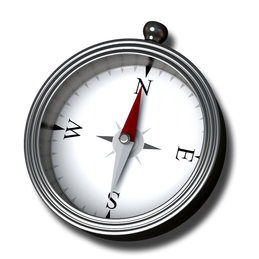
\includegraphics[width=\columnwidth]{img/bussola.png}
\end{figure}
Il magnetismo terrestre permette di orientarsi\\~
\end{column}
\begin{column}{0.3\textwidth}
\visible<2-3>{\begin{figure}
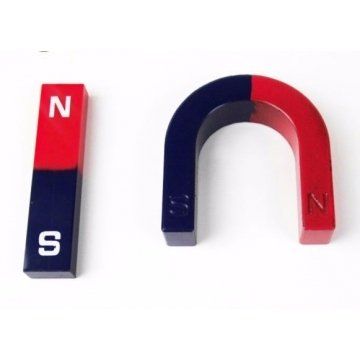
\includegraphics[width=\columnwidth]{img/calamite.jpg}
\end{figure}
I poli delle calamite si possono attrarre o respingere\\~}
\end{column}
\begin{column}{0.3\textwidth}
\visible<3>{\begin{figure}
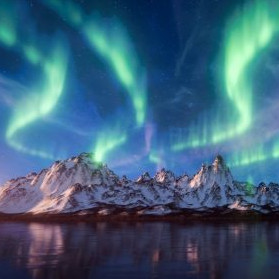
\includegraphics[width=\columnwidth]{img/aurora.jpg}
\end{figure}
L'aurora boreale è conseguenza del magnetismo terrestre}
\end{column}
\end{columns}
\end{frame}

\begin{frame}
\frametitle{Magneti}
\begin{columns}
\begin{column}{0.4\textwidth}
\begin{figure}
\textbf{Magneti naturali}\\~\\~
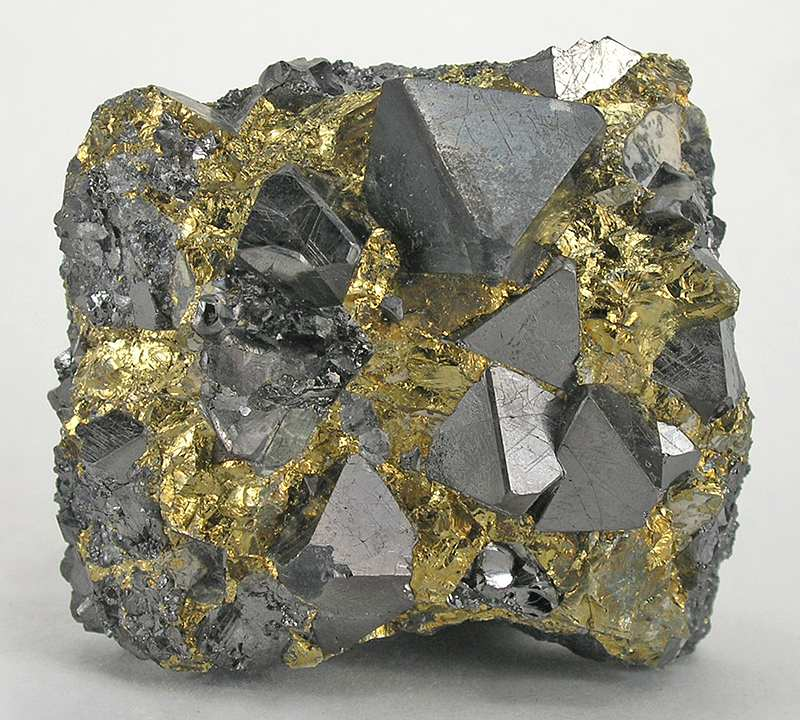
\includegraphics[width=\columnwidth]{img/magnetite.jpg}
Magnetite
\end{figure}
\end{column}
\begin{column}{0.4\textwidth}
\visible<2->{\begin{figure}
\textbf{Magneti artificiali}\\~\\~
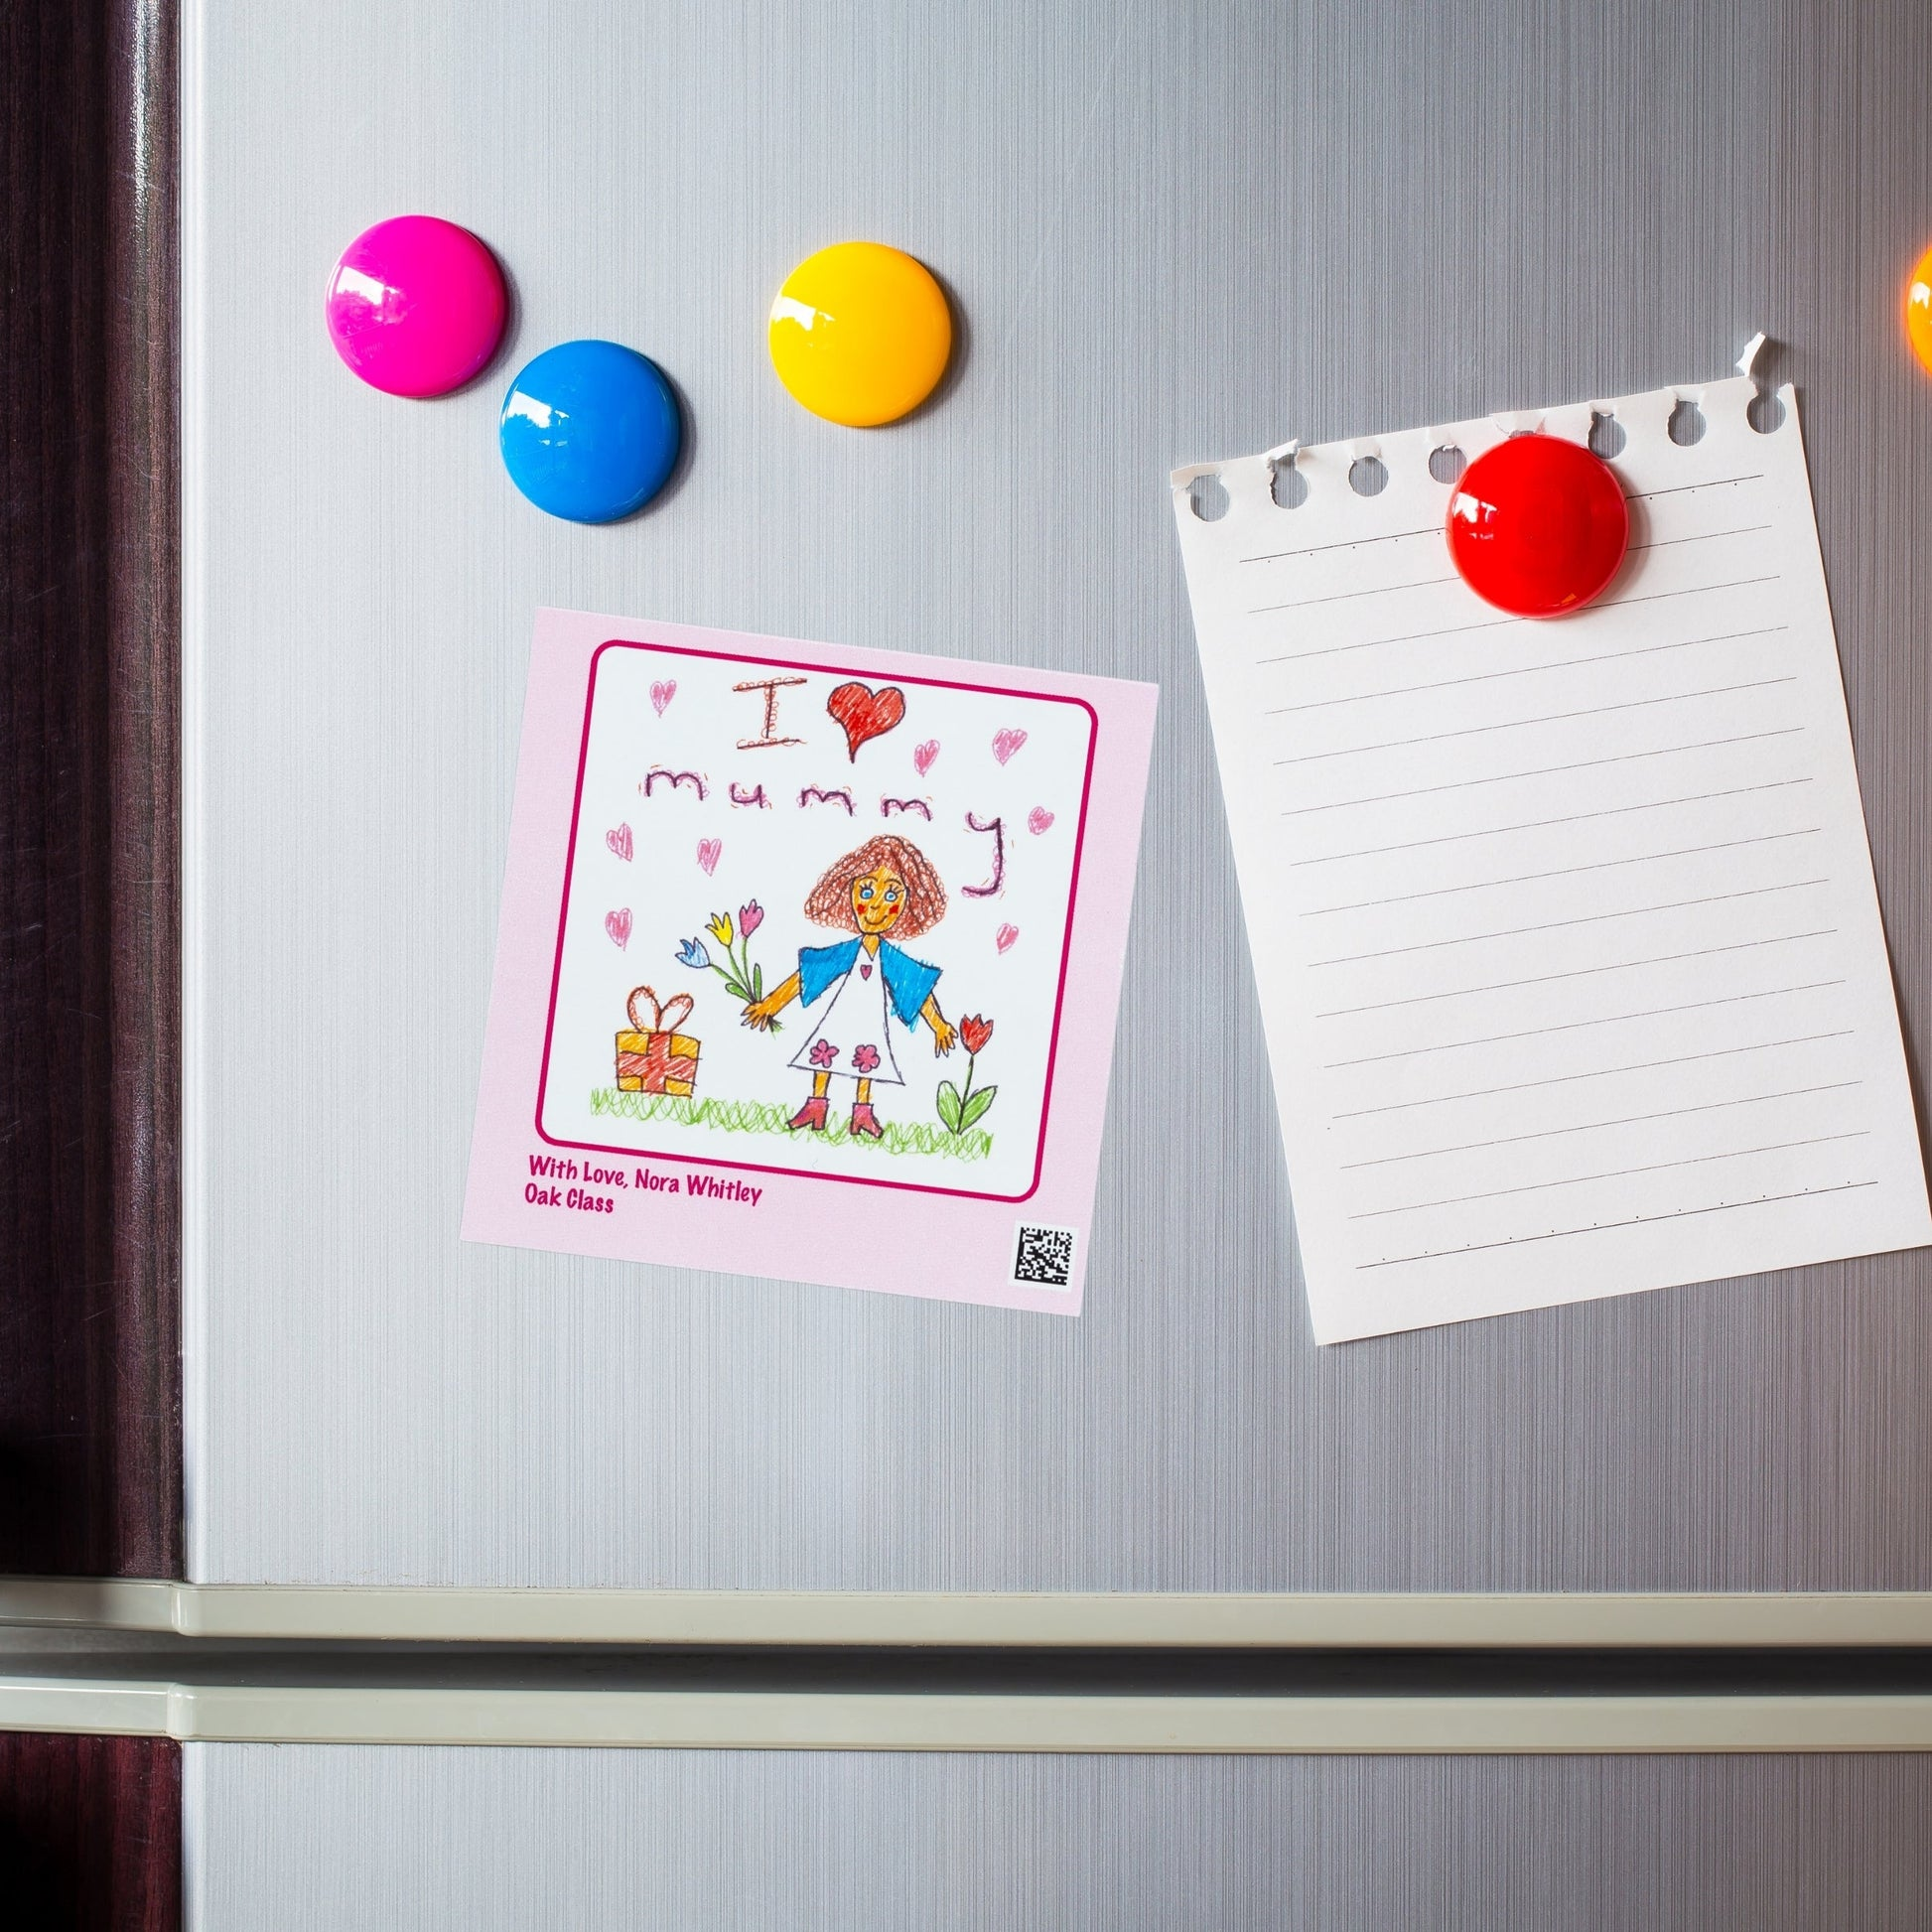
\includegraphics[width=\columnwidth]{img/frigo.jpg}
Calamite
\end{figure}}
\end{column}
\end{columns}
\end{frame}

\begin{frame}
\frametitle{Sostanze ferromagnetiche}
\begin{block}{Definizione}
I materiali che possono essere magnetizzati sono detti \emph{sostanze ferromagnetiche.}
\end{block}\pause

~

Sono ferromagnetici ferro, nichel, cobalto, neodimio e le loro leghe (ad esempio l'acciaio).
\end{frame}



\begin{frame}
\frametitle{Definizione operativa dei poli magnetici}
Una calamita (come l'ago di una bussola) libera di muoversi orienta sempre una sua parte verso un punto in prossimità del polo nord geografico terrestre.\pause

~

Definiamo tale parte della calamita \alert{polo nord} del magnete, l'altro sarà il \alert{polo sud}.
\end{frame}


\begin{frame}
\frametitle{Caratteristiche dei poli magnetici}
Possiamo verificare sperimentalmente che:
\begin{itemize}
  \item \alert<1>{poli dello stesso tipo si respingono}, poli di tipo diverso si attraggono;\pause
  \item i poli magnetici sono \alert{indivisibili}: rompendo una calamita in due parti, si ottengono due calamite!
\end{itemize}
\visible<2->{\begin{figure}
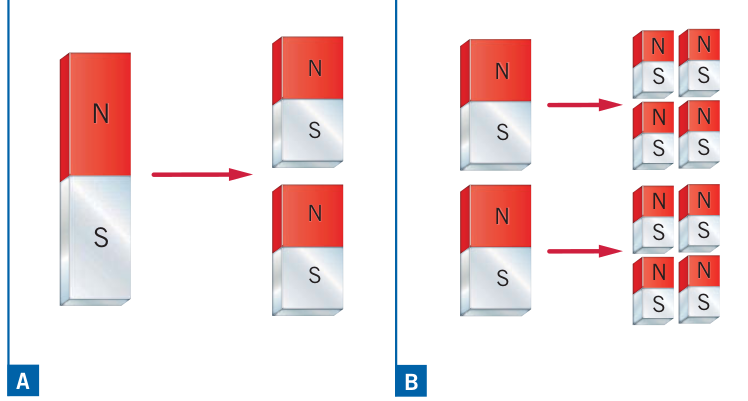
\includegraphics[width=.6\columnwidth]{img/divisionecalamite.png}
\end{figure}}
\end{frame}


\begin{frame}
\frametitle{Campo magnetico}
I magneti interagiscono tra loro generando nello spazio circostante un \alert<1>{campo magnetico}.\pause

~

Il \alert<2>{vettore campo magnetico} si indica con $ \vec{B} $ e si misura in \emph{tesla} $ [T] $.\pause

~

Il \alert<3>{verso positivo del vettore campo magnetico} sarà definito dal polo nord del \emph{magnete di prova}.
\visible<3->{\begin{figure}
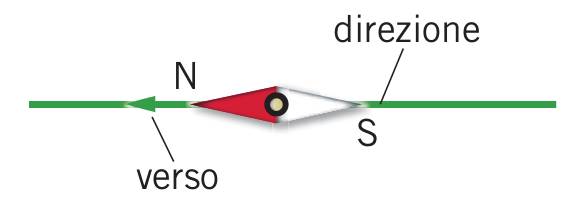
\includegraphics[width=.4\columnwidth]{img/magnetediprova.png}
\end{figure}}
\end{frame}



\begin{frame}
\frametitle{Linee di campo}
Possiamo visualizzare un campo magnetico con le linee di campo, che risultano \alert<1>{uscenti dal polo nord} ed entranti nel polo sud.

~

\begin{figure}
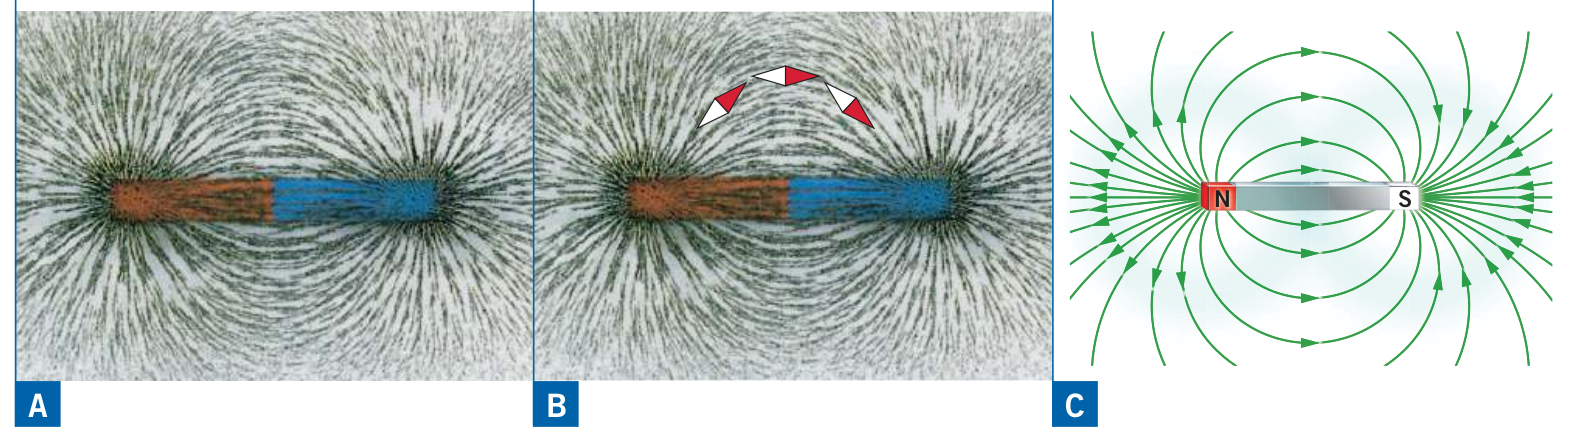
\includegraphics[width=\columnwidth]{img/lineemagnetico.png}
\end{figure}\pause
\alert{$ \vec{B} $ sarà in ogni punto tangente alle linee di campo} e direttamente proporzionale alla loro densità.
\end{frame}


\begin{frame}
\frametitle{Il campo magnetico terrestre}
\begin{figure}
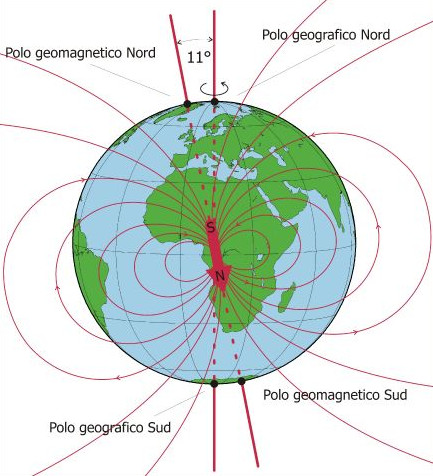
\includegraphics[width=.5\columnwidth]{img/campoterrestre.jpg}
\end{figure}
\end{frame}



\begin{frame}
\frametitle{Confronto con il campo elettrico}
\begin{columns}
\begin{column}{0.5\textwidth}
\begin{figure}
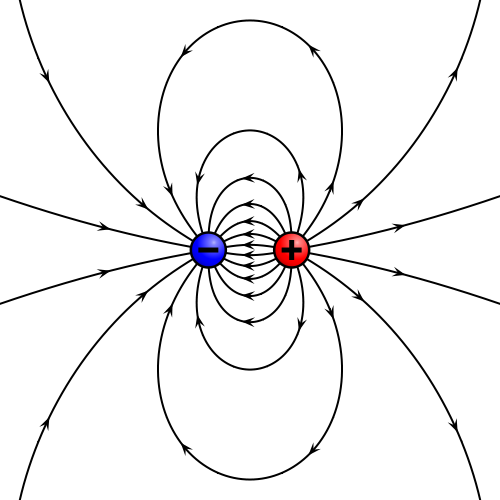
\includegraphics[width=.5\columnwidth]{img/dipoloelettrico.png}
\end{figure}
\visible<2->{Analogie:}
\begin{itemize}
  \item<2-> \alert<2>{sono campi di forza};
  \item<3-> \alert<3>{sono descritti da linee di campo};
  \item<4-> \alert<4>{ci sono due tipi di carica e due poli magnetici};
  \item<5-> \alert<5>{avvengono fenomeni di repulsione e attrazione}.
\end{itemize}
\end{column}
\begin{column}{0.5\textwidth}
\begin{figure}
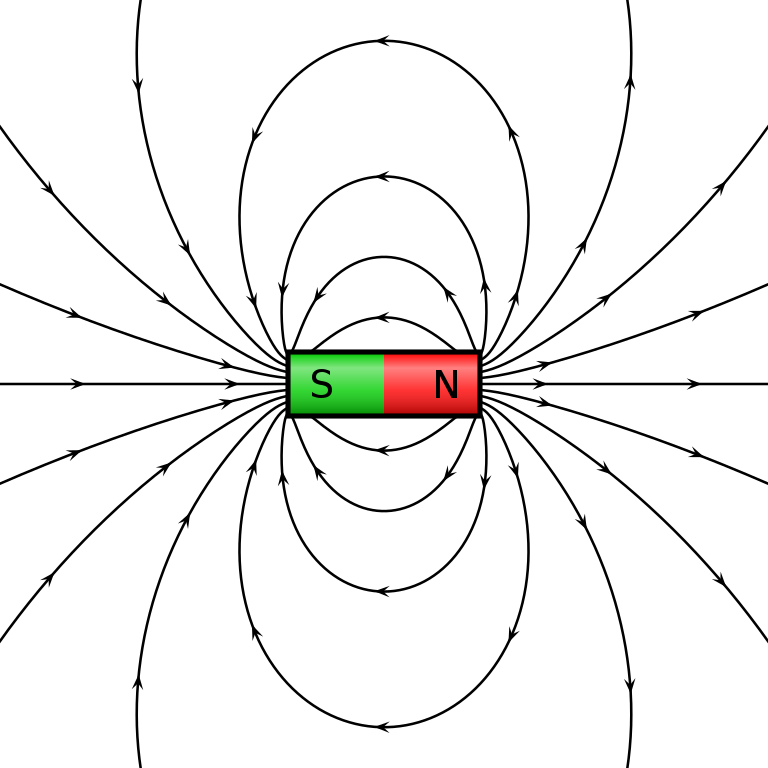
\includegraphics[width=.5\columnwidth]{img/dipolomagnetico.png}
\end{figure}
\visible<6->{Differenze:}
\begin{itemize}
  \item<6-> \alert<6>{le cariche si spostano tra corpi, i poli no};
  \item<7-> \alert<7>{esistono monopoli e dipoli elettrici, ma solo dipoli magnetici};
  \item<8-> \alert<8>{le linee del c.m.~sono sempre chiuse}.
\end{itemize}
\end{column}
\end{columns}
\end{frame}

\section{Interazione}

\begin{frame}
\frametitle{L'esperimento di {\O}rsted (1820)}
Il fisico danese Hans {\O}rsted si accorse che l'ago di una bussola, posto in prossimità di un filo percorso da corrente, \alert<1>{si orienta sempre perpendicolarmente al filo}.\pause

\visible<2->{\begin{figure}
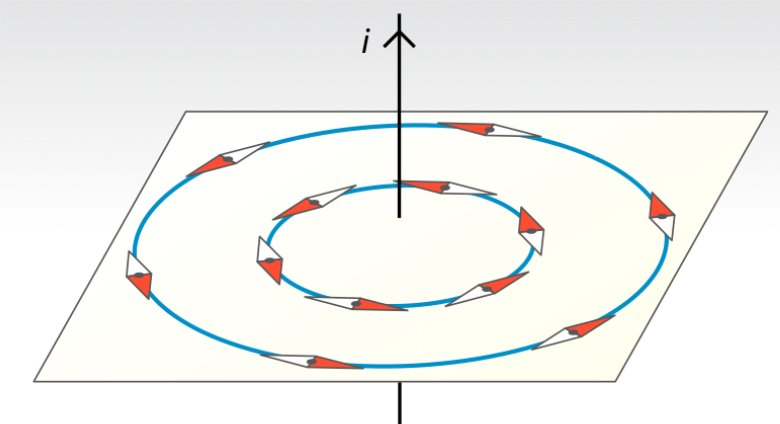
\includegraphics[width=.5\columnwidth]{img/oersted1.jpg}
\end{figure}}\pause
 
Per la prima volta ci si accorse di una \alert{interazione tra fenomeni elettrici e magnetici}.
\end{frame}


\begin{frame}
\frametitle{Campo magnetico di un filo percorso da corrente}
\begin{figure}
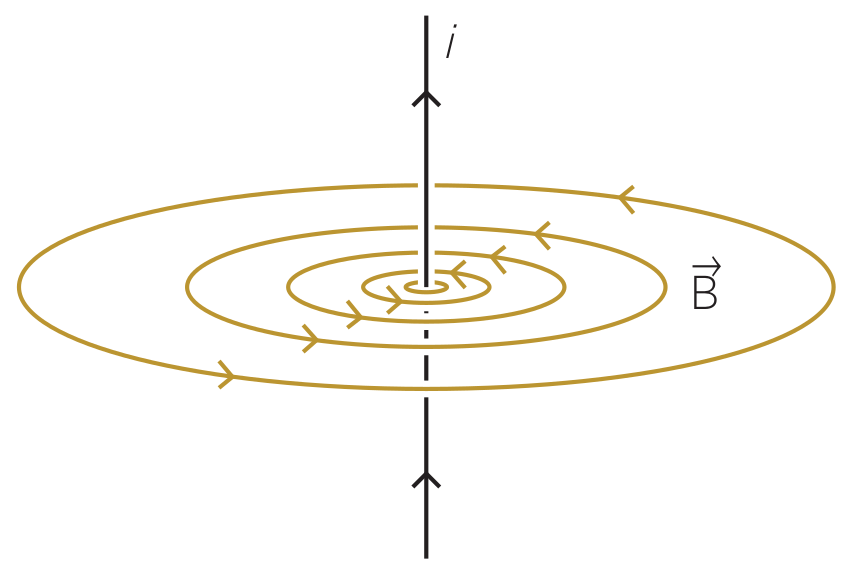
\includegraphics[width=.5\columnwidth]{img/oersted2.png}
\end{figure}
Il campo magnetico generato dal filo:
\begin{itemize}
  \item ha \alert<1>{linee circolari} con centro nel filo che giacciono su piani perpendicolari al filo;\pause
  \item è, in ogni punto dello spazio, \alert<2>{tangente a tali linee};\pause
  \item \alert<3>{diminuisce allontanandosi} dal filo.
\end{itemize}
\end{frame}



\begin{frame}
\frametitle{Verso di rotazione del campo magnetico}
\begin{figure}
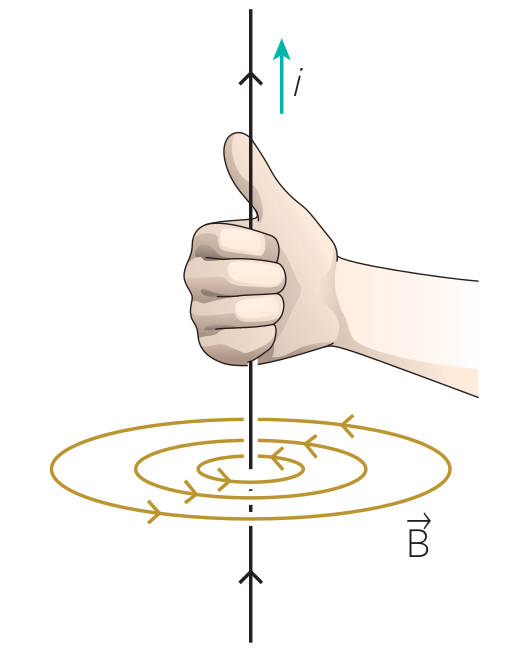
\includegraphics[width=.5\columnwidth]{img/oersted3.png}
\end{figure}
\end{frame}




\begin{frame}
\frametitle{L'esperimento di Faraday (1821)}
\begin{columns}
\begin{column}{0.45\textwidth}
Come possiamo \emph<1>{misurare} l'intensità di $ \vec{B} $?\pause

~

Michael Faraday scopre nel 1821 che un filo percorso da corrente \alert<2>{subisce una forza se immerso in un campo magnetico}.\pause
\end{column}
\begin{column}{0.5\textwidth}
\visible<3>{\begin{figure}
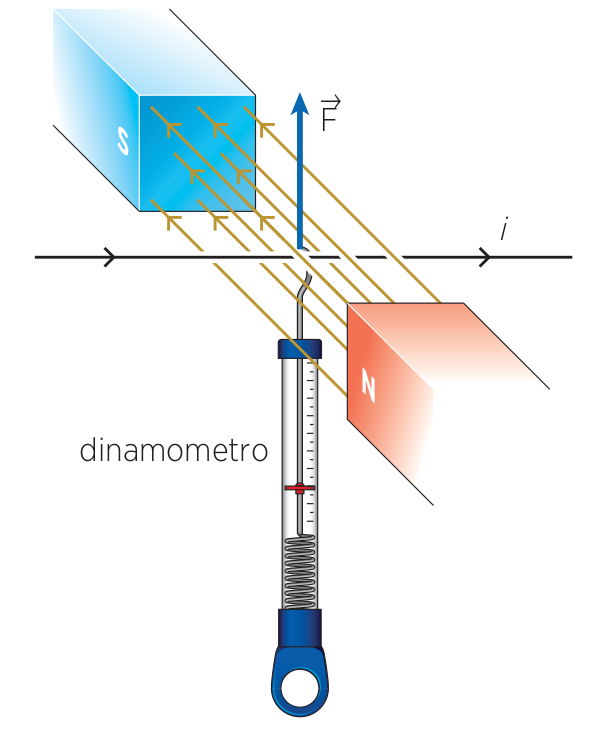
\includegraphics[width=\columnwidth]{img/espfaraday1.png}
\end{figure}}
\end{column}
\end{columns}
\end{frame}



\begin{frame}
\frametitle{Intensità del campo magnetico}
Si vede sperimentalmente che:
\begin{columns}
\begin{column}{0.3\textwidth}
\begin{itemize}
  \item $ F \propto B $;
\end{itemize}
\end{column}
\begin{column}{0.3\textwidth}
\begin{itemize}
  \item $ F \propto i $;
\end{itemize}
\end{column}
\begin{column}{0.3\textwidth}
\begin{itemize}
  \item $ F \propto \ell $.
\end{itemize}
\end{column}
\end{columns}\pause

~

~

Esprimiamo questi fatti definendo l'intensità di $ \vec{B} $ come:
\begin{center}
~~~~~~~~~~~~~~~~~~~~~\colorbox{marroncino!30}{$ B = \dfrac{F}{i\ell} $}\pause~~~~~~~~~$ \left[ T \right] = \left[ \dfrac{N}{A\cdot m} \right] $
\end{center}\pause

~

In particolare, \alert<4>{se il filo e il campo sono perpendicolari la forza è massima e vale:}
\begin{center}
\colorbox{marroncino!30}{$ F=Bi\ell $}
\end{center}
\end{frame}



\begin{frame}
\frametitle{Esempi}
\begin{columns}
\begin{column}{0.4\textwidth}
\begin{figure}
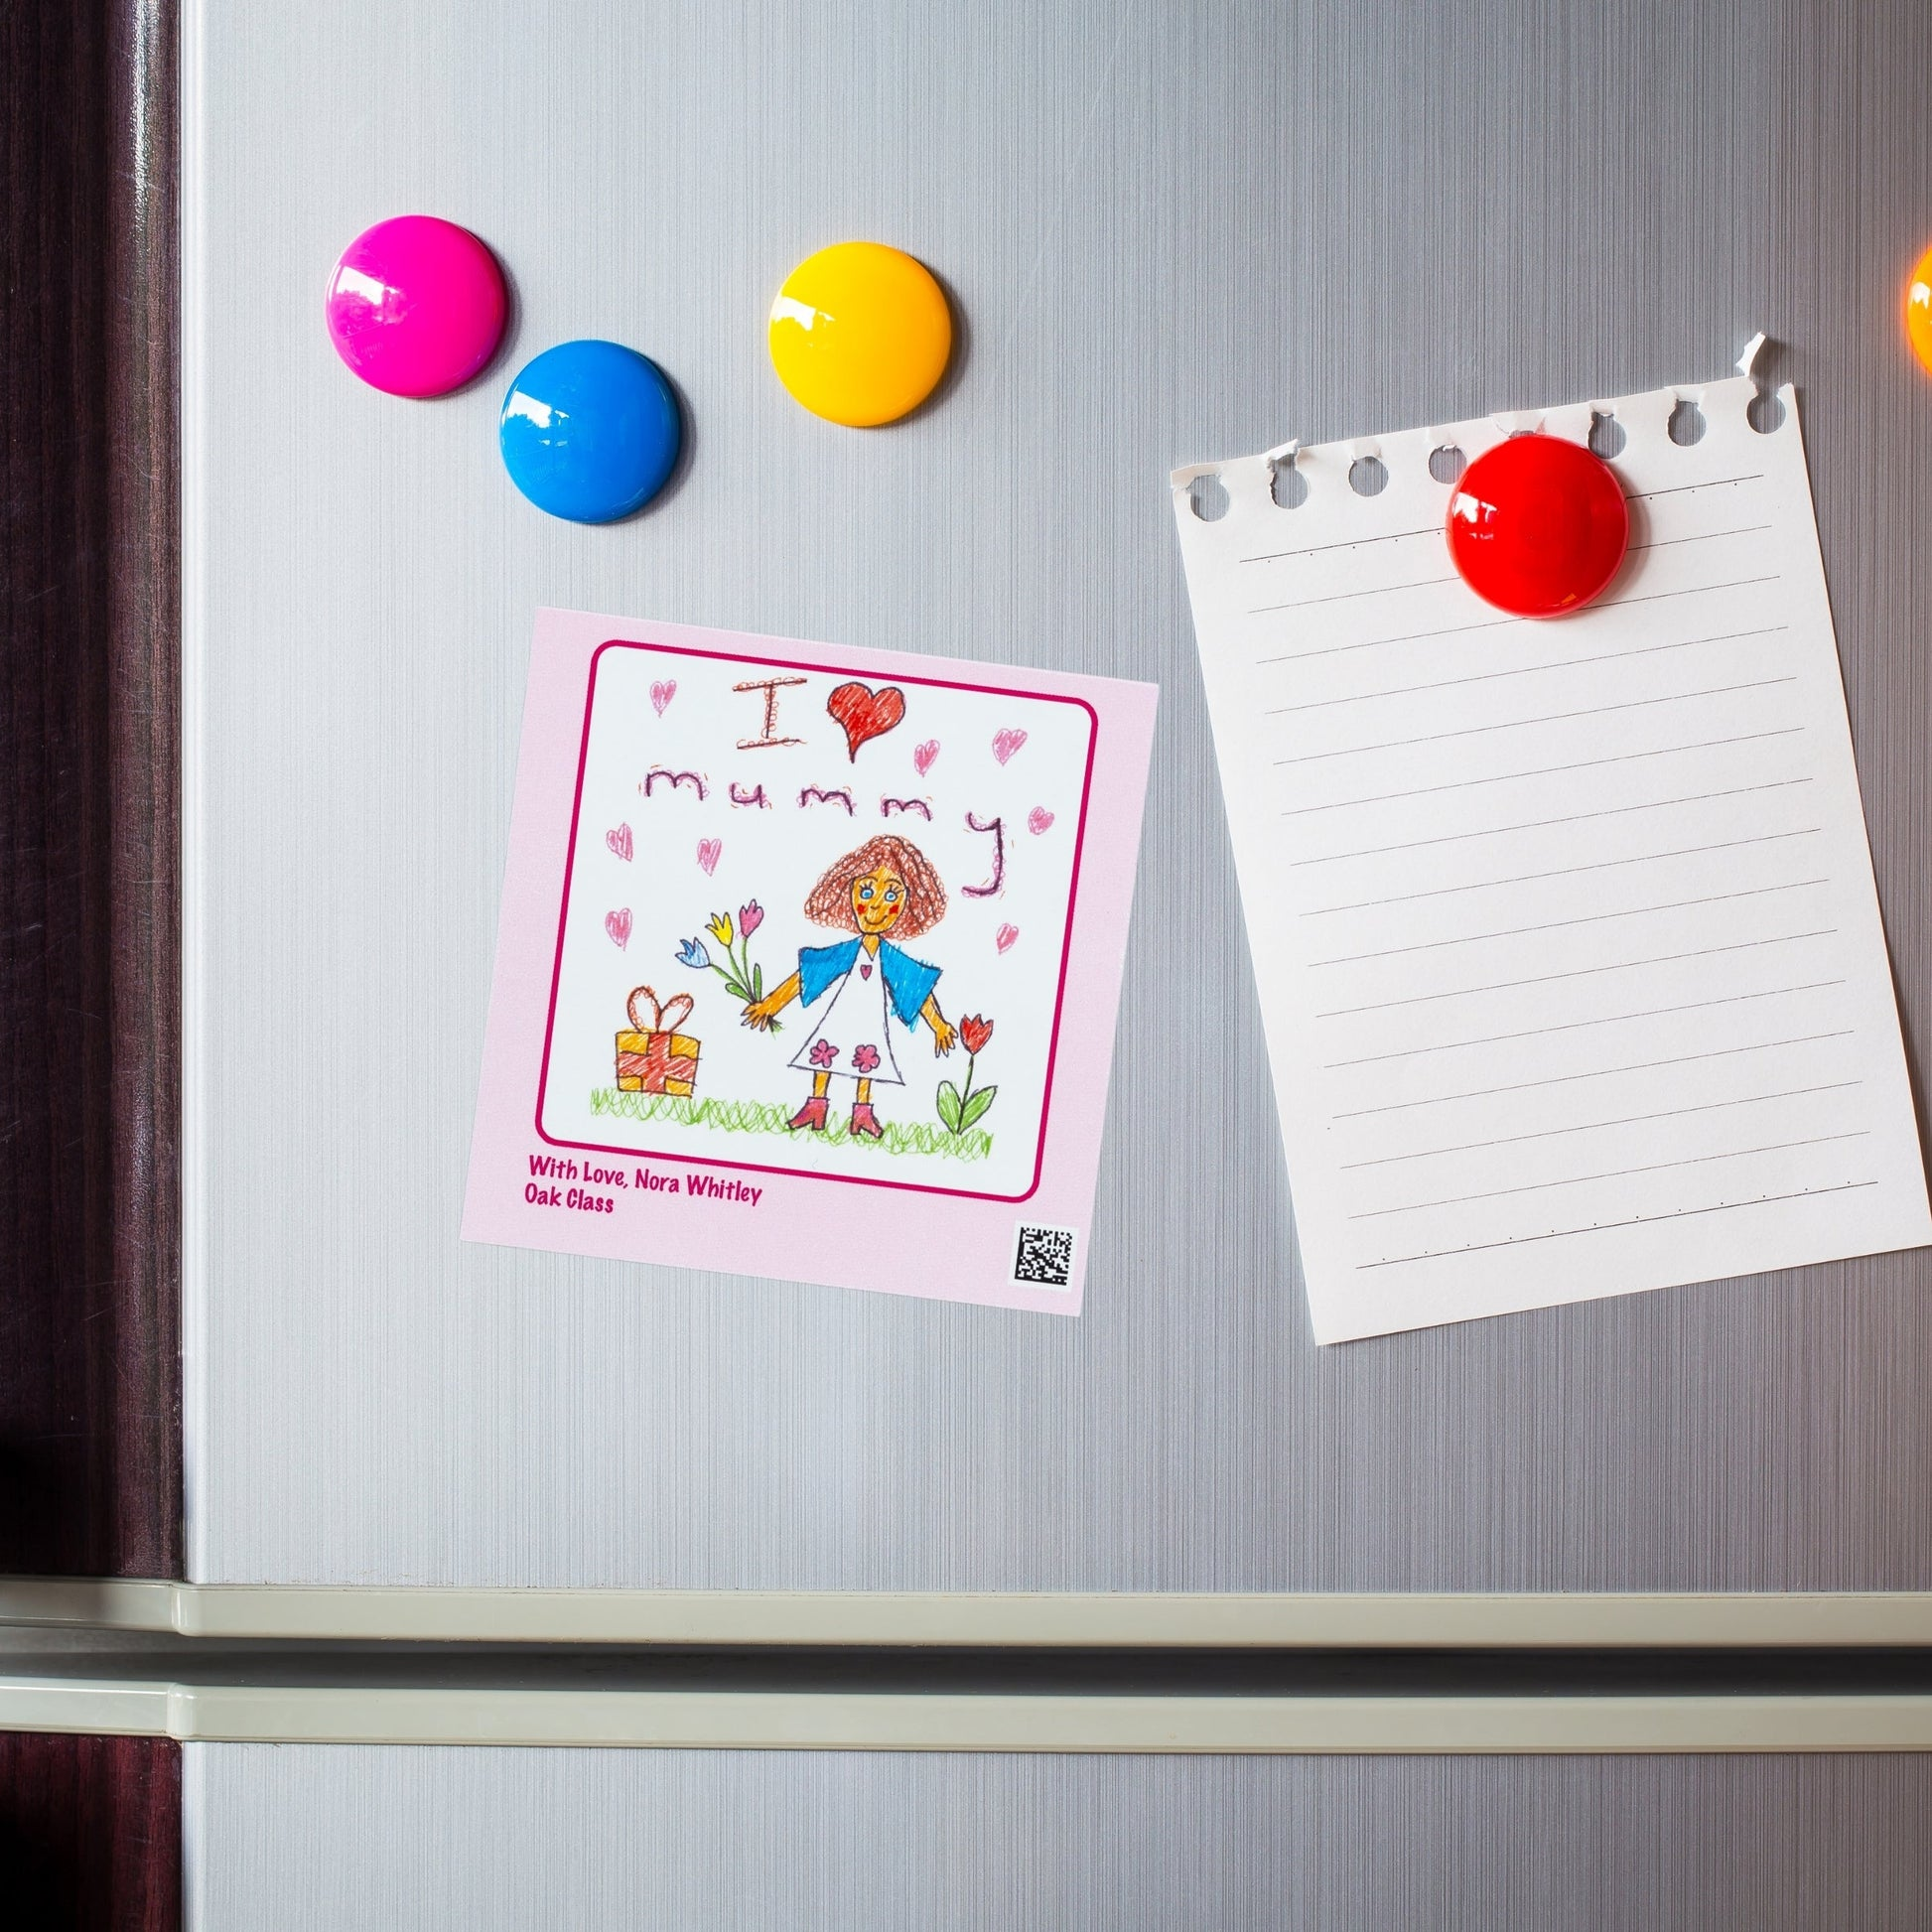
\includegraphics[width=\columnwidth]{img/frigo.jpg}
$ 6 \, mT $
\end{figure}
\end{column}
\begin{column}{0.4\textwidth}
\visible<2->{\begin{figure}
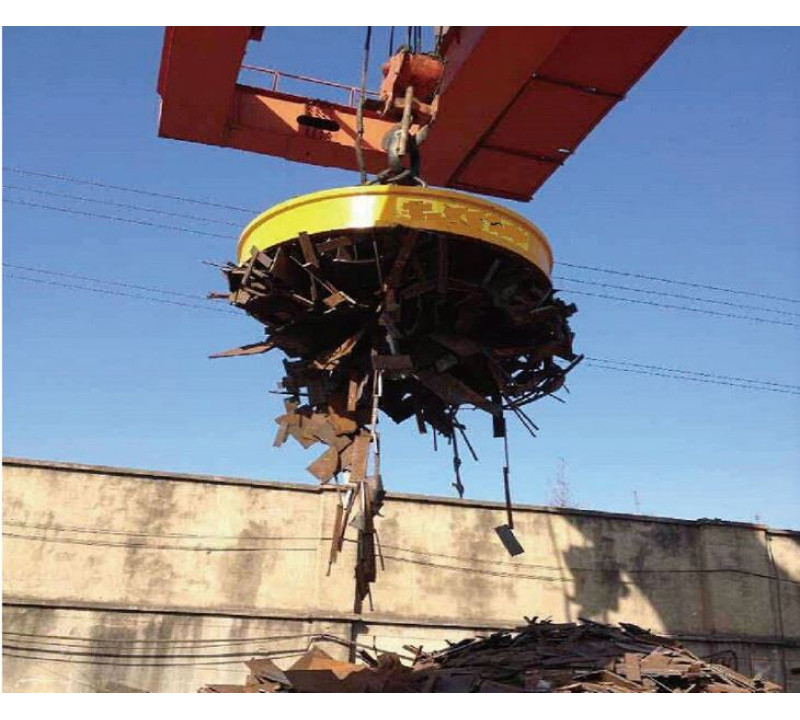
\includegraphics[width=\columnwidth]{img/rottami.jpg}
$ 2 \, T $
\end{figure}}
\end{column}
\end{columns}
\end{frame}





\begin{frame}
\frametitle{Direzione e verso della forza magnetica}
\begin{figure}
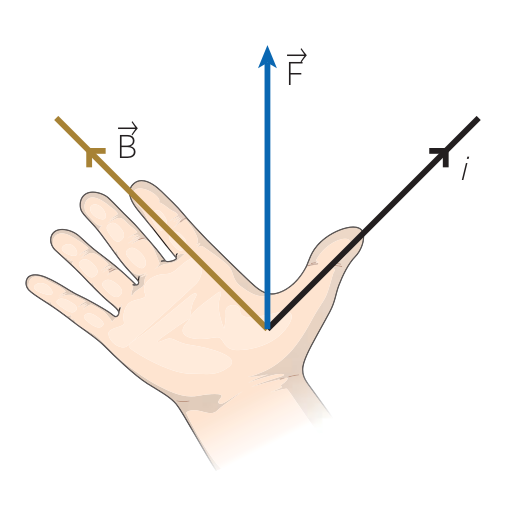
\includegraphics[width=.5\columnwidth]{img/espfaraday2.png}
\end{figure}
\end{frame}


\begin{frame}
\frametitle{Esercizio}
\begin{exampleblock}{Intensità del campo magnetico}
  Un filo lungo $ 50 \, cm $, percorso da una corrente di $ 7,23 \times 10^{-3} \, A $, è immerso in un campo magnetico uniforme di intensità $ B $ e si trova nella posizione per cui la forza che agisce su di esso è massima e pari a $ 3,2 \, N $.

  ~

  Quanto vale $ B $?\hspace{\fill}[$ 8,9 \times 10^{2} \, T $]
\end{exampleblock} 
\end{frame}




\begin{frame}
\frametitle{L'esperimento di Ampère (un settimana dopo \O rsted)}
\begin{columns}
\begin{column}{0.4\textwidth}
Sappiamo:
\begin{itemize}
  \item da \O rsted, che \alert<1>{una corrente genera un campo magnetico};\pause
  \item da Faraday, che \alert<2>{una corrente subisce una forza magnetica}.\pause
\end{itemize}

~

Conclusione: \alert<3>{due fili percorsi da corrente eserciteranno una forza l'uno sull'altro}.
\end{column}
\begin{column}{0.5\textwidth}
\visible<3->{\begin{figure}
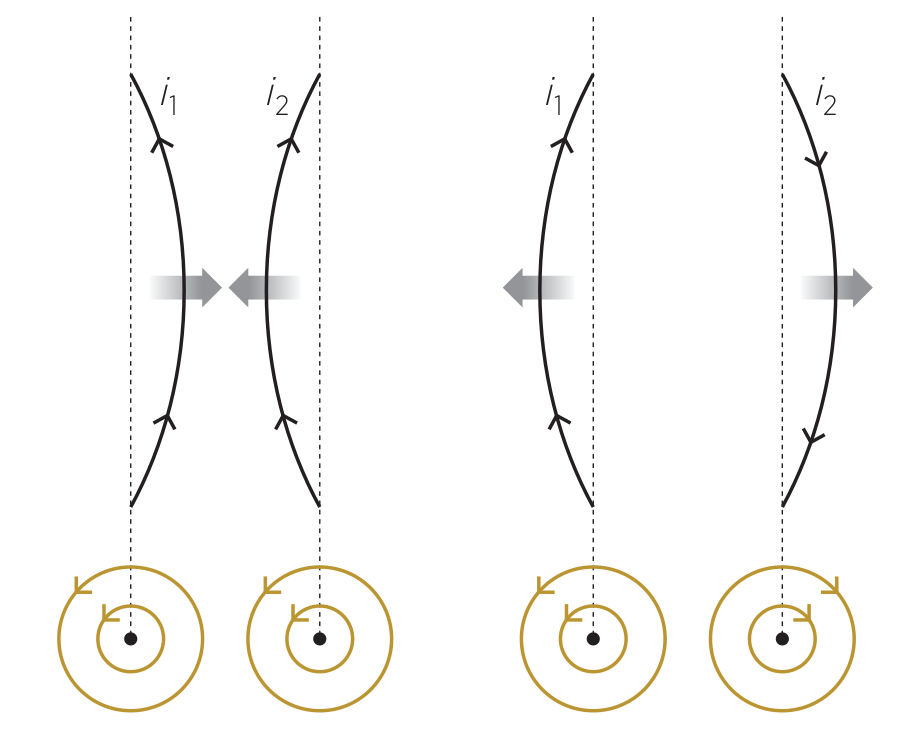
\includegraphics[width=\columnwidth]{img/espampere.png}
\end{figure}}
\end{column}
\end{columns}
\end{frame}

\begin{frame}
\frametitle{Legge di Ampère}
Si verifica sperimentalmente che:
\begin{columns}
\begin{column}{0.3\textwidth}
\begin{itemize}
  \item $ F \propto i_1, i_2 $;
\end{itemize}
\end{column}
\begin{column}{0.3\textwidth}
\begin{itemize}
  \item $ F \propto \ell $;
\end{itemize}
\end{column}
\begin{column}{0.3\textwidth}
\begin{itemize}
  \item $ F \propto \dfrac{1}{d} $.
\end{itemize}
\end{column}
\end{columns}\pause

~

~

Otteniamo pertanto la legge:
\begin{center}
\colorbox{marroncino!30}{$ F = \dfrac{\mu_0}{2\pi} \cdot \dfrac{i_1i_2}{d}\ell $}
\end{center}
con:
\begin{center}
\colorbox{marroncino!30}{$ \mu_0 = $ permeabilità magnetica del vuoto $ = 4\pi \times 10^{-7} \, \dfrac{N}{A^2} $}
\end{center}
\end{frame}


\begin{frame}
\frametitle{Esercizio}
\begin{exampleblock}{Forza magnetica}
  In due lunghi fili conduttori rettilinei, che distano tra loro $ 2,2 \, cm $, sono presenti due correnti di intensità $ 3,8 \, A $ e $ 7,5 \, A $.

  ~

  Qual è il valore della forza magnetica che agisce su un tratto di filo lungo $ 2,0 \, m $?\hspace{\fill}[$ 5,2 \times 10^{-4} \, N $]
\end{exampleblock} 
\end{frame}


\begin{frame}
\frametitle{Legge di Biot-Savart}
\begin{figure}
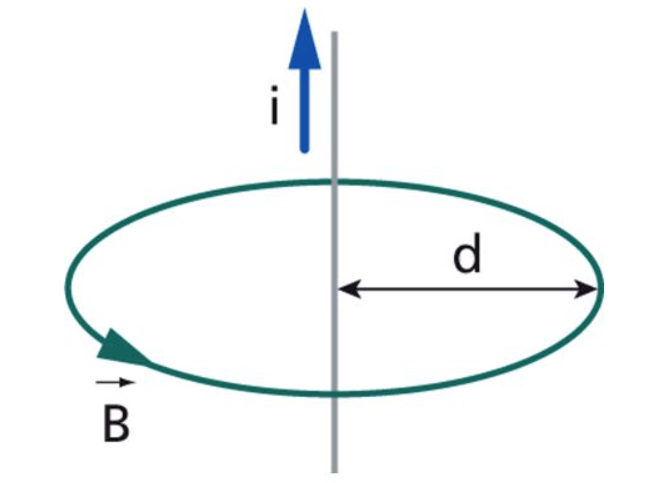
\includegraphics[width=.4\columnwidth]{img/biotsavart.png}
\end{figure}
Un filo percorso da corrente $ i $ genera a distanza $ d $ un campo magnetico di intensità:
\begin{center}
\colorbox{marroncino!30}{$ B = \dfrac{\mu_0}{2\pi} \cdot \dfrac{i}{d} = \mu_0 \cdot \dfrac{i}{2\pi d} $}
\end{center}
\end{frame}



\begin{frame}
\frametitle{Esercizio}
\begin{exampleblock}{Distanza dal filo}
  Alcuni pacemaker sono dotati di un interruttore magnetico che viene pilotato dall'esterno attraverso un campo magnetico. Per poter agire sul pacemaker, il campo deve avere un'intensità di $ 5 \times 10^{-4} \, T $. Tale campo viene generato tramite un filo percorso da corrente di intensità $ 1.2 \times 10^{3} \, A $ che è posizionato dal medico ad una distanza $ d $ dal paziente.

  ~

  Calcola il valore della distanza $ d $.\hspace{\fill}[$ 0,5 \, m $]
\end{exampleblock} 
\end{frame}




\section{Motore}


\begin{frame}
\frametitle{Cosa hanno in comune?}
\begin{columns}
\begin{column}{0.3\textwidth}
\begin{figure}
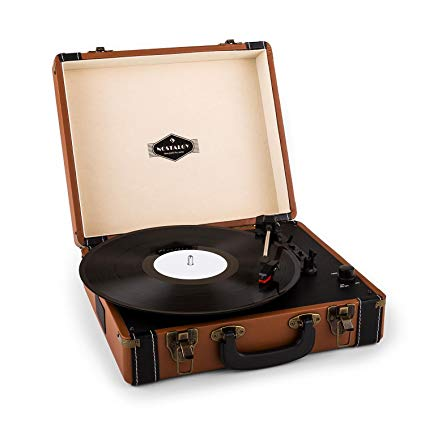
\includegraphics[width=\columnwidth]{img/giradischi.jpg}
\end{figure}
\end{column}
\begin{column}{0.3\textwidth}
\visible<2-3>{\begin{figure}
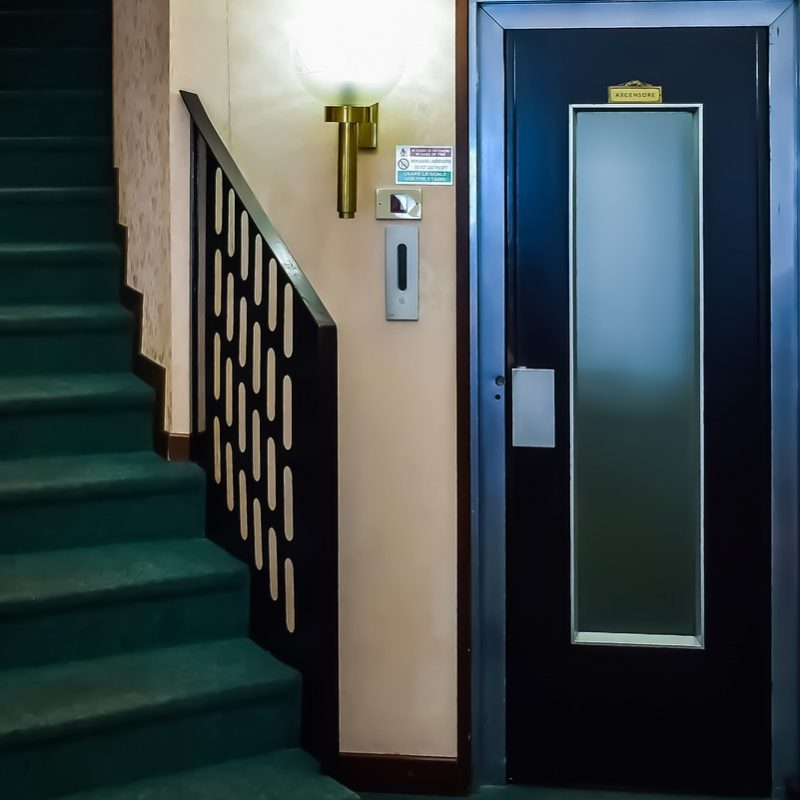
\includegraphics[width=\columnwidth]{img/ascensore.jpg}
\end{figure}}
\end{column}
\begin{column}{0.3\textwidth}
\visible<3>{\begin{figure}
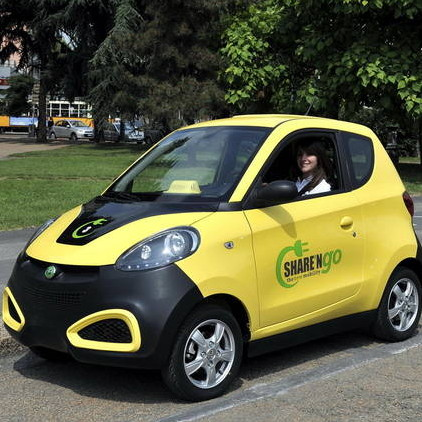
\includegraphics[width=\columnwidth]{img/autoelettrica.jpg}
\end{figure}}
\end{column}
\end{columns}
\end{frame}



\begin{frame}
\frametitle{Trasformazione di energia}
\begin{block}{Motore elettrico}
Un motore elettrico è un dispositivo che trasforma energia elettrica in energia meccanica.
\end{block}
\begin{columns}
\begin{column}{0.4\textwidth}
\visible<2->{\begin{figure}
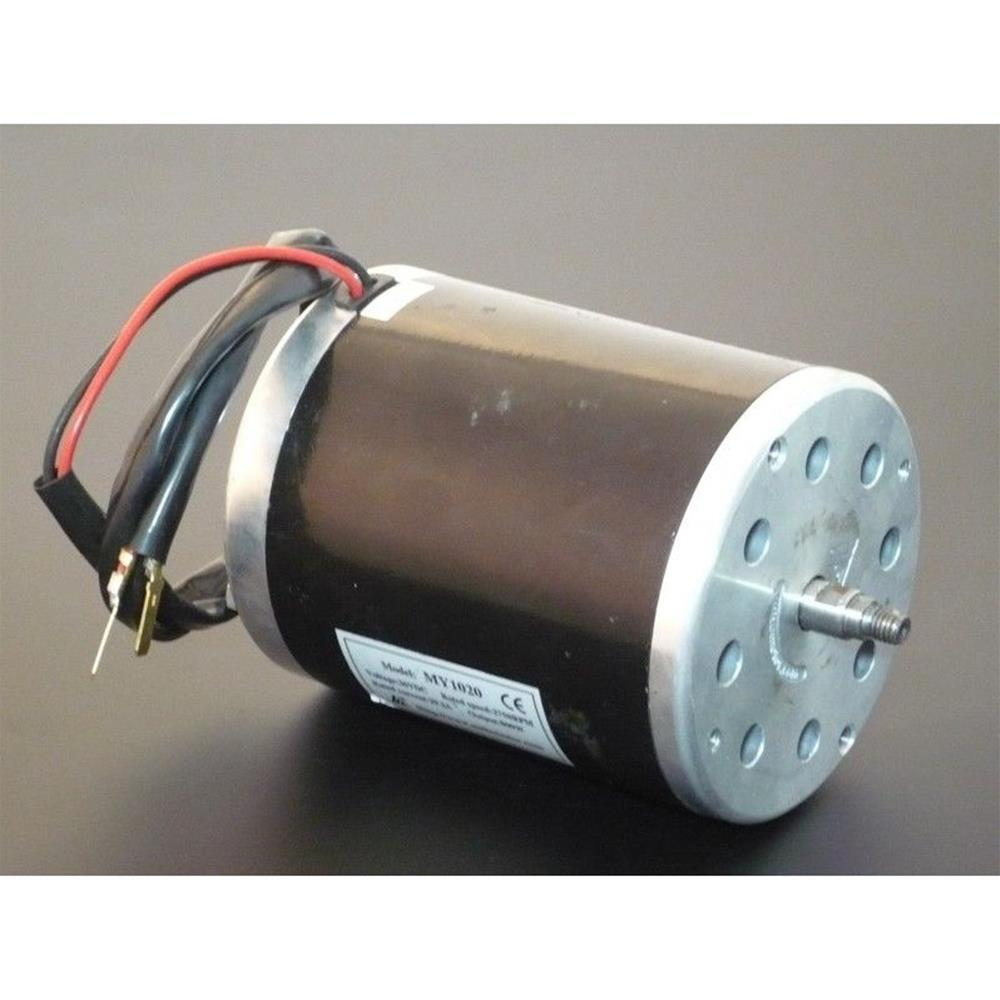
\includegraphics[width=\columnwidth]{img/motore1.jpg}
\end{figure}}
\end{column}
\begin{column}{0.4\textwidth}
\visible<3->{\begin{figure}
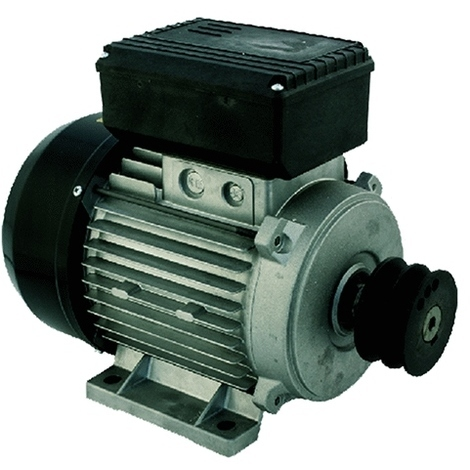
\includegraphics[width=\columnwidth]{img/motore2.jpg}
\end{figure}}
\end{column}
\end{columns}
\end{frame}

\begin{frame}
\frametitle{Modello di un motore elettrico}
\begin{figure}
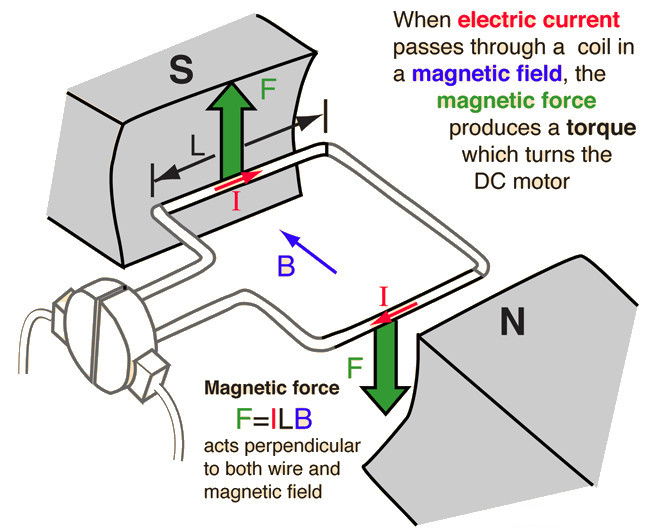
\includegraphics[width=.7\columnwidth]{img/schemamotore.jpg}
\end{figure}
\end{frame}


\begin{frame}
\frametitle{Modello di un motore elettrico (2)}
Il moto della spira dura finché essa non si dispone perpendicolarmente al campo.\pause

~

Le forze non tendono più a farla ruotare, ed è pertanto necessario invertire il verso della corrente, grazie ai \alert{commutatori ad anelli}.

~

\begin{center}
\href{video/Motoreelettrico.mp4}{\beamergotobutton{Video: Funzionamento di un motore elettrico}}
\end{center}
\begin{center}
\href{gif/motoreelettrico.gif}{\beamergotobutton{GIF: Funzionamento di un motore elettrico}}
\end{center}\pause
\begin{block}{Inversione della corrente}
Cambiando il verso della corrente ogni mezzo giro, la coppia di forze mantiene la spira in rotazione.
\end{block}
\end{frame}




\section{Lorentz}

\begin{frame}
\frametitle{Forza magnetica senza filo}
Sappiamo:
\begin{itemize}
  \item da \O rsted, che \alert<1>{una corrente genera un campo magnetico};\pause
  \item da Faraday, che \alert<2>{una corrente subisce una forza magnetica}.\pause
\end{itemize}

~

È possibile verificare che :
\begin{itemize}
  \item \alert<3>{qualsiasi carica in moto genera un campo magnetico};\pause
  \item \alert<4>{qualsiasi carica in moto subisce una forza magnetica}.\pause
\end{itemize}

~

Ciò che vediamo accadere alle correnti (nei fili) è l'effetto macroscopico di tali fenomeni.
\end{frame}


\begin{frame}
\frametitle{Dimostrazione}
Ricordiamo:
\begin{center}
$ F = i\ell B $\pause ~~~~~~~~~~~~~~ $ i = \dfrac{\Delta q}{\Delta t} $
\end{center}\pause

~

Immaginiamo una carica $ q $ che si muove, in un tempo $ \Delta t $, in un tratto di filo lungo $ \ell $.\pause
\begin{center}
$ F = \dfrac{q}{\Delta t} \ell B =\pause q\left(\dfrac{\ell}{\Delta t} \right)B $ 
\end{center}\pause
Il termine tra parentesi è \alert<6>{$ v $, la velocità della carica}.
\end{frame}


\begin{frame}
\frametitle{La forza di Lorentz}
\begin{block}{Forza di Lorentz}
Una carica $ q $, in moto con velocità $ v $ in un campo $ B $, subisce una forza:
\begin{center}
\colorbox{marroncino!30}{$ F = q v B $}
\end{center}
\end{block}
\end{frame}



\begin{frame}
\frametitle{Regola della mano destra (attenzione!)}
\begin{columns}
\begin{column}{0.4\textwidth}
\visible<1->{\begin{figure}
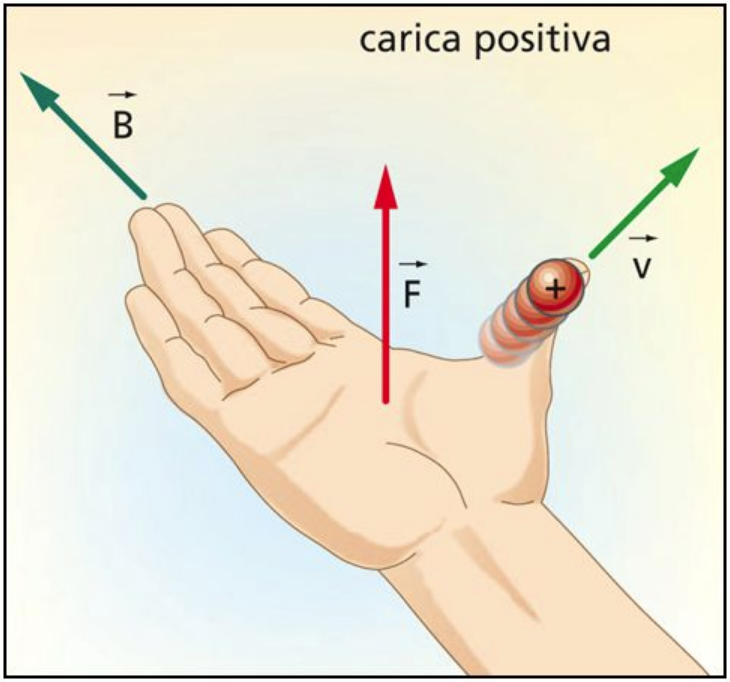
\includegraphics[width=\columnwidth]{img/lorentz1.png}
\end{figure}}
\end{column}
\begin{column}{0.4\textwidth}
\visible<2->{\begin{figure}
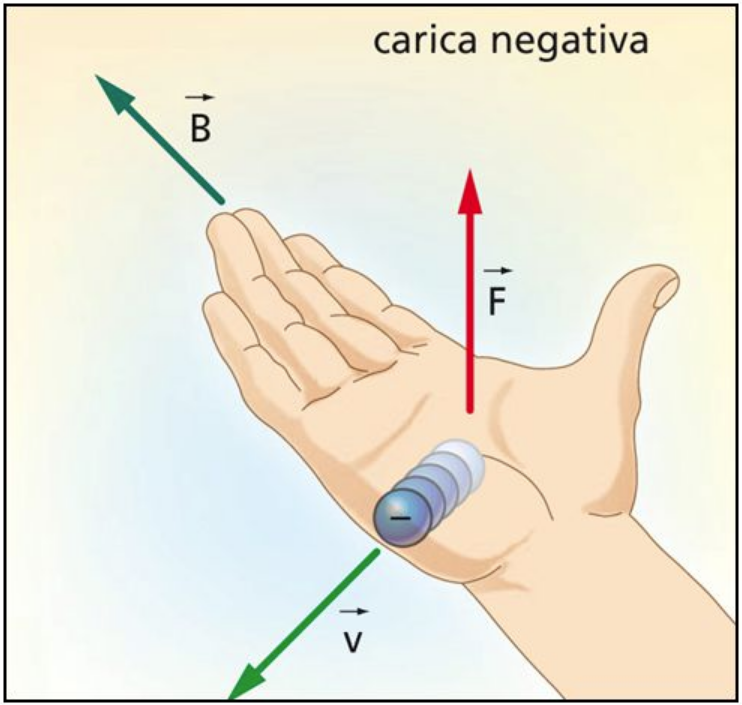
\includegraphics[width=\columnwidth]{img/lorentz2.png}
\end{figure}}
\end{column}
\end{columns}
\end{frame}

\begin{frame}
\frametitle{Esercizio}
\begin{exampleblock}{Moto di un protone}
  Un protone si muove in un campo magnetico uniforme di intensità $ 1,0 \times 10^{-2} \, T $, in una direzione perpendicolare a quella del campo magnetico. Sul protone agisce una forza di modulo $ 1,6 \times 10^{-16} \, N $.

  ~

  Calcola il modulo della velocità del protone.\hspace{\fill}[$ 1,0 \times 10^{5} \, \frac{m}{s} $]
\end{exampleblock} 
\end{frame}


\begin{frame}
\frametitle{Forza centripeta}
Quando una forza agisce su un corpo, questo viene accelerato: 
\begin{center}
$ \vec{F} = m\vec{a} $
\end{center}\pause

~

Se la forza è perpendicolare alla velocità del corpo, essa agisce da forza centripeta e abbiamo un \alert<2>{moto circolare uniforme}.
\begin{center}
\href{gif/centripeta.gif}{\beamergotobutton{GIF: Forza centripeta e moto circolare}}
\end{center}\pause

~

\alert<3>{La fdL, quando agisce su una carica, ne causa un moto circolare!}
\begin{center}
\href{video/Motomagnetico.mp4}{\beamergotobutton{Video: Moto di una carica in un campo magnetico}}
\end{center}
\end{frame}


\begin{frame}
\frametitle{Aurora boreale}
\begin{figure}
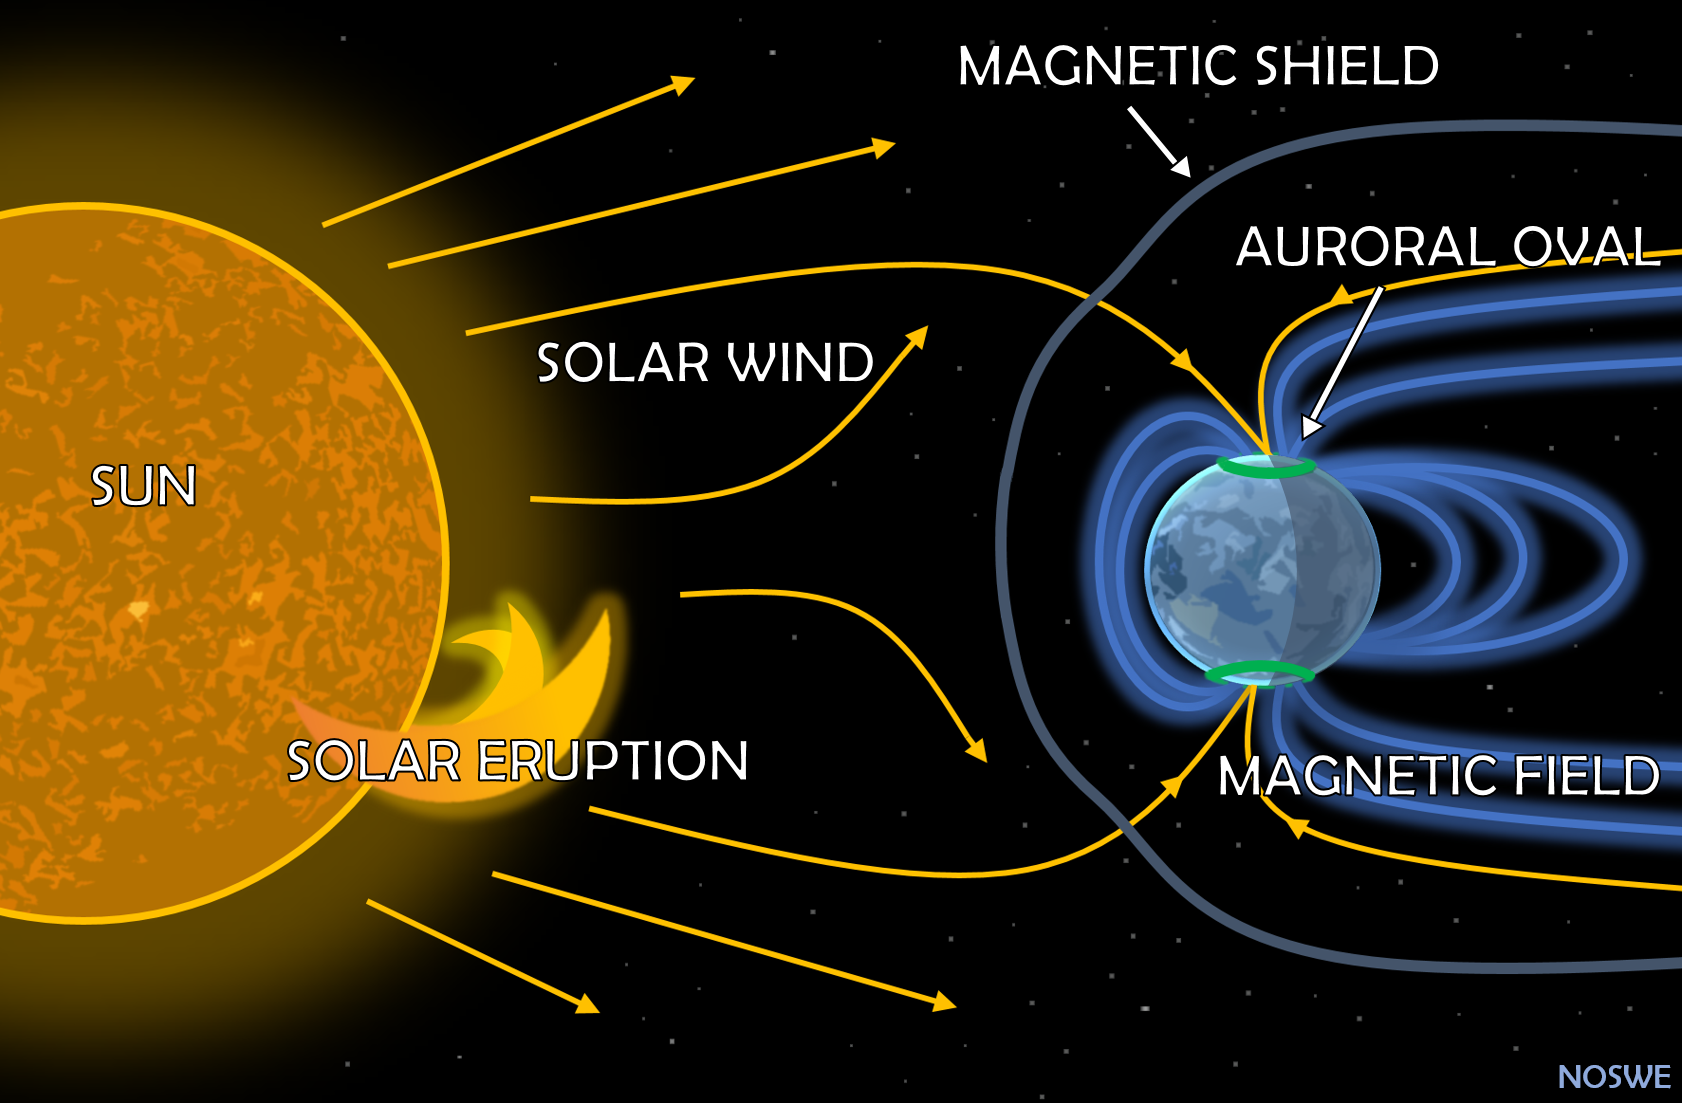
\includegraphics[width=\columnwidth]{img/ventosolare.png}
\end{figure}
\end{frame}


\section{Flusso}

\begin{frame}
\frametitle{Flusso  del campo magnetico}
Il flusso di $ \vec{B} $ attraverso una superficie $ S $ (eventualmente gaussiana) si definisce in modo analogo a quello di $ \vec{E} $. 
\begin{center}
\colorbox{marroncino!30}{$ \Phi_{S}(\vec{B}) = \vec{B} \cdot \vec{S} = BS\cos\theta $}
\end{center}\pause
Il flusso del campo magnetico si misura in \emph{weber}:
\begin{center}
$ [Wb] = [T\cdot m^2] $
\end{center}
\end{frame}


\begin{frame}
\frametitle{Il teorema di Gauss per il campo magnetico}
\begin{block}{Teorema di Gauss per il campo magnetico}
Il flusso del campo magnetico attraverso una superficie chiusa (gaussiana) è uguale a zero.
\begin{center}
\colorbox{marroncino!30}{$ \Phi_S (\vec{B}) = 0 $}
\end{center}
\end{block}\pause
Esistono cariche elettriche isolate, ma non monopòli magnetici (poli nord o sud isolati): \alert{per ogni linea di campo uscente ci sarà una linea di campo entrante}.
\end{frame}


\begin{frame}
\frametitle{Confronto tra i due teoremi di Gauss}
\begin{figure}
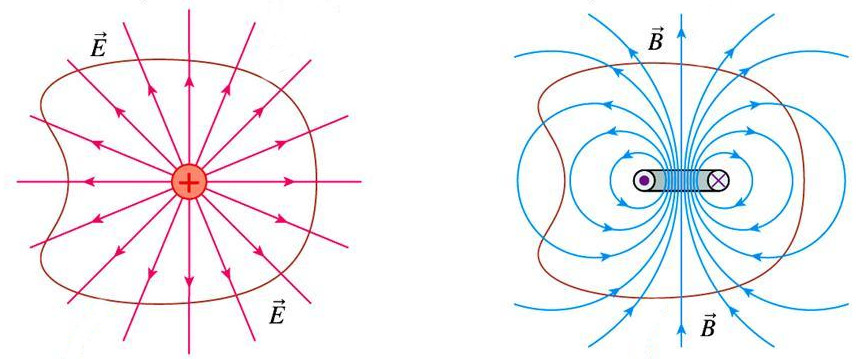
\includegraphics[width=\columnwidth]{img/confrontogauss.jpg}
\end{figure}
\end{frame}




\end{document}
